\begin{figure}
    \begin{subfigure}{\columnwidth}
    \centering
    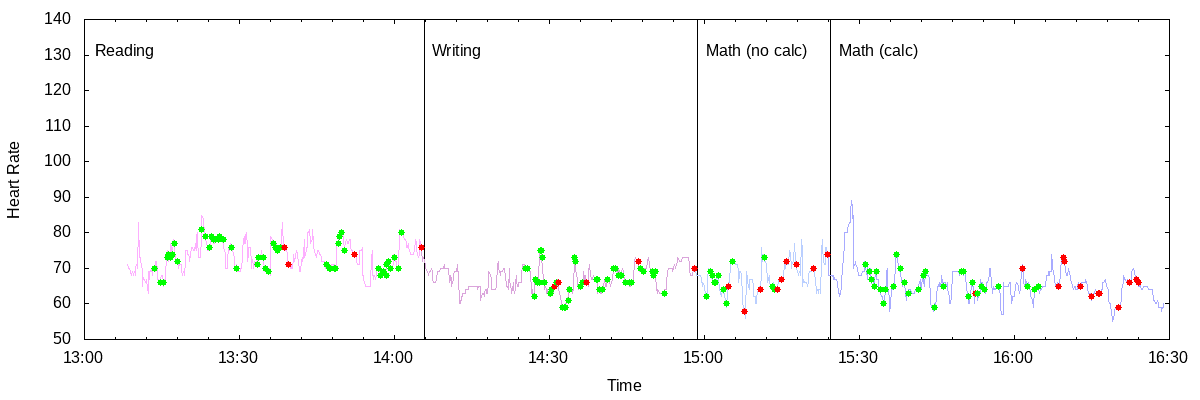
\includegraphics[width=1\columnwidth]{figs/images/graph_s17.png}
    \caption{The heartrate graph over time for one exam from student s17.}
    \label{fig:s17}
    \end{subfigure}
    
    \begin{subfigure}{\columnwidth}
    \centering
    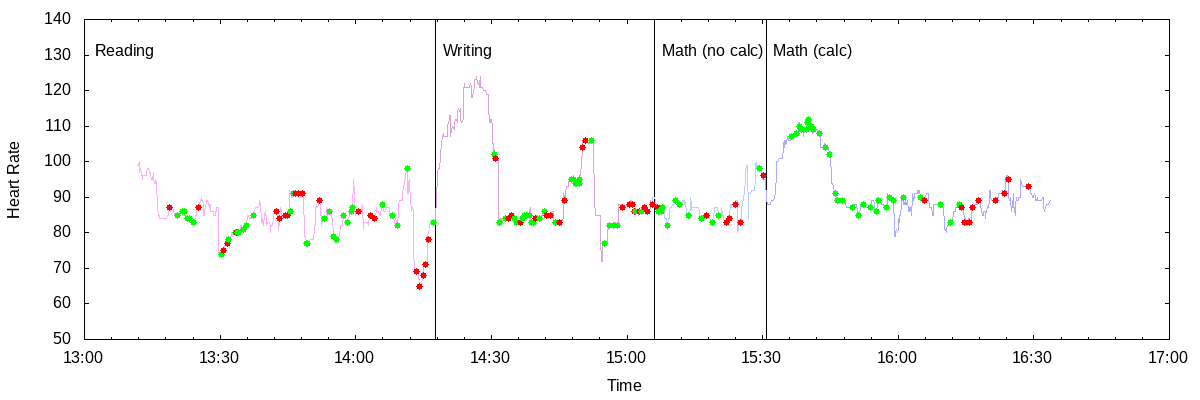
\includegraphics[width=1\columnwidth]{figs/images/graph_s3.png}
    \caption{The heartrate graph over time for one exam from student s3.}
    \label{fig:s3}
    \end{subfigure}
    
    \caption{Two graphs showing students' heartrate during an exam. Green dots indicate time points where the student entered a correct answer, while red dots indicate the student entered an incorrect answer.}
    \label{fig:hearrate_graphs}
\end{figure}

